\chapter{Аналитический раздел}
\section{Анализ предметной области}

\subsection{Понятие рекомендательных алгоритмов}
Пусть рассматриваются предметы, представленные какими-либо данными и пользователи, которые их используют.
Пользователи присваивают предметам оценки в соответствии со своими субъективными предпочтениями.
Оценкой является число из определённого множества или отрезка.
Считается, что чем выше оценка, тем предмет субъективно нужнее пользователю.
Далее рассмотрена одна из постановок цели рекомендательной системы.
Необходимо предсказать оценки, которые выбранный пользователь присвоит новым для него предметам, после чего сформировать список предметов, которые данный пользователь определит как субъективно нужные~\cite{aggarwal}.
Таким образом, объект исследования -- рекомендательные системы -- это программы, которые информируют пользователя о субъективно нужных для него объектах.

\subsection[Формализация задачи рекомендательных\\систем]{Формализация задачи рекомендательных систем}
Рассматривается постановка задачи рекомендательных алгоритмов.
Пусть:
\begin{itemize}
    \item $U$ -- множество пользователей программы;
    \item $X$ -- множество из $M$ объектов, с которыми взаимодействуют пользователи;
    \item $W_i \subset X$ -- множество объектов, которые оценил пользователь $u_i$, где $i \in \overline{1, N}$, $N$ -- количество пользователей;
    \item $\alpha_{i,j}$ -- оценка объекта $X_j$ пользователем $U_i$, где $X_j \in W_i, i \in \overline{1, N}$.
\end{itemize}
Матрицей оценок называется матрица $Y$ размером $N \times M$, где элемент $y_{i,j}$ строки $i$ и столбца $j$ содержит либо оценку пользователя $U_i$ для объекта $X_j$, либо метку о её отсутствии~\cite{aggarwal}.
Также матрица оценок может содержать неявные оценки объектов пользователем, принимающие значения $0$ и $1$.
Такие оценки собираются автоматически во время работы рекомендательной системы.
Входными данными является следующее:
\begin{itemize}
    \item матрица оценок;
    \item матрица неявных оценок;
    \item данные об объектах.
\end{itemize}
Необходимо выбрать из множества $X \setminus W_i$ один или несколько объектов таким образом, чтобы его оценка пользователем $U_i$ была максимальна~\cite{aggarwal}.
Таким образом, выходными данными является список объектов $x_i \in X$, отсортированный по убыванию предполагаемой оценки от пользователя.
\section{Методы коллаборативной фильтрации}

В данном разделе рассмотрены методы рекомендаций рецептов, учитывающие только оценки пользователей.
Также приведён метод гибридной фильтрации, учитывающий ещё и содержание рецептов.

\subsection{Простая коллаборативная фильтрация}
Коллаборативная фильтрация позволяет предсказать оценку, которую даст выбранный пользователь какому-либо рецепту, на основе оценок других пользователей~\cite{segaran}.
Оценка пользователя представляет собой число в пределах $[a, b]$.

Пусть:
\begin{itemize}
    \item $N$ -- количество пользователей;
    \item $R_i$ -- множество рецептов, оценённых пользователем $u_i$, $i \in \overline{1, N}$;
    \item $u'$ -- пользователь, оценки которого необходимо предсказывать;
    \item $R'$ -- множество рецептов, которое оценил пользователь $u'$.
\end{itemize}

Вычисляется коэффициент подобия между пользователями $u'$ и $u_i$ для $i \in \overline{1, N}$.
Для этого выполняются следующие действия:
\begin{itemize}
    \item находится пересечение $R$ множеств $R'$ и $R_i$;
    \item собираются векторы оценок $a, b$, где $a_k, b_k$ -- оценки пользователей $u', u$ соответственно для рецепта $R_k, k \in \overline{1, |R|}$;
\end{itemize}
Таким образом, $\gamma = F(a, b)$.
В качестве метрики $F$ обычно выступает Евклидово расстояние или коэффициент корреляции Пирсона~\cite{segaran}.
Евклидово расстояние вычисляется по формуле~\cite{segaran}:
\begin{equation}
    F(a, b) = \sqrt{\sum\limits_{i=1}^{n} (a_i - b_i)^2},
    \label{eq:dist}
\end{equation}
а коэффициент корреляции Пирсона -- по формуле~\cite{segaran}:
\begin{equation}
    F(a, b) = \dfrac{\sum\limits_{i=1}^{n} a_i b_i - \dfrac{\left(\sum\limits_{i=1}^{n} a_i\right) \left(\sum\limits_{i=1}^{n} b_i\right)}{n}}{\sqrt{\left(\sum\limits_{i=1}^{n} a_i^2 - \dfrac{\left(\sum\limits_{i=1}^{n} a_i\right)^2}{n}\right) \left(\sum\limits_{i=1}^{n} b_i^2 - \dfrac{\left(\sum\limits_{i=1}^{n} b_i\right)^2}{n}\right)}}
\end{equation}
где $n = |a| = |b|$.

Пусть:
\begin{itemize}
    \item $\alpha_k, k \in \overline{1, M}$ -- оценка пользователя $u'$ для каждого рецепта, где $M$ -- количество рецептов;
    \item $I_k$ -- множество номеров пользователей, оценивших рецепт $k, k \in \overline{1, M}$;
    \item $\beta_{k,i}$ -- оценка рецепта $k$ пользователем $i$, $k \in \overline{1, M}, i \in I_k$;
    \item $\alpha_k$ -- оценка пользователя $u'$ для рецепта c номером $k$.
\end{itemize}
Тогда $\alpha_k$ рассчитывается по формуле~\cite{segaran}:
\begin{equation}
    \alpha_k = \frac{\sum\limits_{i \in I_k} (\gamma_i\beta_{k,i})}{\sum\limits_{i \in I_k} (\gamma_i)}.
\end{equation}
Таким образом на основе оценок других пользователей предсказывается оценка выбранного пользователя.

К особенностям данного метода относится необходимость в хранении матрицы оценок рецептов, где элемент в строке $i$ и столбце $j$ содержит либо оценку пользователя $i$ для рецепта $j$, либо метку о том, что оценка отсутствует.
Заполнение такой матрицы является трудоёмкой задачей и должно происходить заранее~\cite{segaran}.

Коллаборативная фильтрация имеет следующий ряд особенностей~[1]:
\begin{itemize}
    \item нельзя применить к пользователю, данные о котором отсутствуют;
    \item используется только матрица предпочтений и данные об оценках пользователя;
    \item метод не позволяет выявить новых предпочтений у пользователя, так как основан на истории его оценок.
\end{itemize}

\subsection{Матричные разложения}
В рассматриваемом методе делается предположение, что пользователи и объекты описываются вектором скрытых признаков, представленных в виде чисел.
Причём скалярное произведение вектора пользователя на вектор объекта даёт оценку, которую данный пользователь поставил этому объекту~\cite{yandex_matrix}.
Вводятся обозначения:
\begin{itemize}
    \item $X, Y$ -- матрицы размерностью $T \times N$ и $T \times M$ соответственно;
    \item $x_u, y_i$ -- столбцы $u, i$ матриц $X, Y$ соответственно, являющиеся представлением пользователя $u$ и объекта $i$;
    \item $R$ -- множество пар $(u, i)$ индексов пользователя и объекта, таких что оценка пользователя $u$ для объекта $i$ известна;
    \item $r$ -- матрица предпочтений, где $r_{u,i}$ оценка, которую пользователь $u$ выставил объекту $i$, $u \in \overline{1, N}, i \in \overline{1, M}$.
\end{itemize}
Оценка пользователем $u$ объекта $i$ вычисляется по формуле~\cite{yandex_matrix}:
\begin{equation}
    \hat{r}_{u,i} = x_u^Ty_i.
\end{equation}
Задача заключается в нахождении скрытых признаков.
Следовательно, необходимо минимизировать функцию потерь, в качестве которой выступает~\cite{yandex_matrix}:
\begin{equation}
    L(X, Y) = \sum_{(u, i) \in R}{(r_{ui} - \hat{r}_{u,i})^2}.
\end{equation}
Таким образом задача рекомендаций сведена к задачи оптимизации.
Тогда следует применить $L2$-регуляризацию, чтобы не произошло переобучение модели~\cite{yandex_matrix}.
После применения $L2$-регуляризации, функция потерь принимает вид:
\begin{equation}
    L(X, Y) = \sum_{(u, i) \in R}{(r_{ui} - \hat{r}_{u,i})^2} + \lambda \sum_{u = 1}^{N}{(||x_u||^2C_u)} + \lambda \sum_{i = 1}^{M}{(||y_i||^2C_i)},
    \label{eq:loss}
\end{equation} где $\lambda > 0$, а $C=(C_1,\dots,C_N)$ -- вектор констант.

Алгоритм минимизации функции потерь~\eqref{eq:loss} состоит из следующих шагов~\cite{yandex_matrix}:
\begin{itemize}
    \item начинается цикл вычислений до тех пор, пока функция потерь не примет достаточно маленькое значение;
    \item фиксируется матрица $X$;
    \item решается задача $L2$-регуляризованной регрессии для поиска матрицы $Y$;
    \item фиксируется матрица $Y$;
    \item решается задача $L2$-регуляризованной регрессии для поиска матрицы $X$;
    \item вычисляется новое значение функции потерь и выполняется переход в начало цикла.
\end{itemize}

Далее рассмотрен шаг алгоритма вычисления строки $x_u$ матрицы $X$.
Необходимо найти такое значение вектора $x_u$, для которого значение функции потерь~\eqref{eq:loss} минимально.
Тогда значение $x_u$ может быть представлено как~\cite{yandex_matrix}:
\begin{equation}
    \underset{x_u}{argmin} \sum_{(u, i) \in R}{(r_{ui} - x_u^Ty_i)^2} + \lambda \sum_{u = 1}^{N}{(||x_u||^2C_u)} + \lambda \sum_{i = 1}^{N}{(||y_i||^2C_i)},
    \label{eq:argmin_step_1}
\end{equation}
где функция $\underset{x_u}{argmin}$ обозначает такое $x_u$, при котором значение выражения минимально.
Выражение~\eqref{eq:argmin_step_1} упрощается~\cite{yandex_matrix}:
\begin{equation}
    \underset{x_u}{argmin} -2x_u^T\sum_{(u, i) \in R}{(r_{ui}y_i)} + x_u^T(\sum_{(u, i) \in R}{(y_iy_i^T) + \lambda C_uI})x_u,
    \label{eq:argmin_step_2}
\end{equation}
где $I$ -- единичная матрица.
Далее применяется следующее соотношение~\cite{yandex_matrix}:
\begin{equation}
    \underset{x_u}{argmin} -2x_u^TB + x_u^TAx_u = A^{-1}B.
    \label{eq:th1}
\end{equation}
Из~\eqref{eq:argmin_step_2}--\eqref{eq:th1} следует, что
\begin{equation}
    x_u = (\sum_{i: (u, i) \in R}{(y_iy_i^T)}+ \lambda C_uI)^{-1}\sum_{i: (u, i) \in R}{(r_{u,i}y_i)}.
\end{equation}

\subsection{Гибридные рекомендательные методы}
Существуют алгоритмы рекомендаций, которые предсказывают оценку объекта пользователем на основе как матрицы оценок, так и его параметров.
Вводятся следующие обозначения:
\begin{itemize}
    \item $U = (u_i | i \in \overline{1,k})$ -- кортеж рассматриваемых пользователей;
    \item $u' \notin U$ -- пользователь, для которого необходимо сделать рекомендацию;
    \item $p_i, i \in \overline{1, n}$ -- вектор из $m$ параметров объекта $i$, который оценил пользователь $u'$;
    \item $r_i, i \in \overline{1,n}$ -- вектор, где $r_{i,j}, j \in \overline{1,k}$ -- оценка объекта $i$ пользователем $u_j$;
    \item $y$ -- вектор, где $y_i, i \in \overline{1,n}$ -- оценка объекта $i$ пользователем $u'$.
\end{itemize}
Создаётся матрица $X$, строка $i$ которой является конкатенацией векторов $p_i$ и $r_i$.
Аналогично для объектов, не оценённых $u'$, строится матрица $X'$.
Необходимо на основании данных $X, y$ найти вектор $y'$, где $y'_i$ -- оценка для объекта, представляемого вектором $X'_i$.
Для этого разрабатывается модель $M$, в результате обучения которой на данных $(X, y)$ вектор $y'$ вычисляется по формуле $y' \approx M(X')$~\cite{segaran}.
В качестве такой модели выступает одна из следующих~\cite{segaran}:
\begin{itemize}
    \item решающее дерево;
    \item линейная регрессия;
    \item $K$ ближайших соседей;
    \item логистическая регрессия;
    \item нейросеть.
\end{itemize}

Более того, допустимо комбинировать перечисленные модели для получения составной~\cite{segaran}.
Пусть есть $N$ моделей $M_1,\dots,M_N$, обученные на данных $(X, y)$.
В результате их применения к $X$ получаются результаты $q_1,\dots,q_N$, которые являются вариантами вектора $y$.
Аналогично $M_i(X') = q'_i, i \in \overline{1,N}$.
Таким образом, появляется необходимость в разработке другой модели $M_0$, которая после обучения на данных $(q_1,\dots,q_N,y)$ используется для вычисления $y'$ по формуле $y' \approx M_0(q'_1,\dots,q'_N)$.
Алгоритм работы всей составной модели содержит следующие шаги~\cite{segaran}:
\begin{itemize}
    \item принять на вход матрицу параметров объектов $X'$;
    \item вычислить $q_i = M_i(X'), i \in \overline{1,N}$;
    \item вычислить $y' = M_0(q_1,\dots,q_N)$.
\end{itemize}
Таким образом, получается комбинация моделей для наиболее точного предсказания оценок объектов выбранным пользователем.

Далее рассмотрены особенности гибридного рекомендательного метода.
Рассмотренный метод сводит задачу рекомендаций к задаче машинного или глубокого обучения.
Это позволяет разработать несколько различных моделей и выбрать наиболее точную из них в результате тестирования.
Под точностью подразумевается значение функции потерь, которая вводится для оценки качества модели на тестовом наборе данных.
Также гибридный метод рекомендаций способен использовать наиболее полный набор данных, что повышает точность результатов.
Но при этом не предусматривается решение проблемы <<холодного старта>>, которая заключается в том, что если пользователь новый, что и данных о его оценках либо относительно мало, либо нет вообще.
Таким образом, модель для рекомендаций обучается на меньшем количестве данных, что сказывается на точности рекомендаций.
Другая сложность гибридного рекомендательного метода заключается в том, что вектора с оценками $r_i, i \in \overline{1,n}$ разрежены, так как каждый объект вероятнее всего не оценён каждым пользователем $i \in \overline {1,k}$.
Таким образом, данные, на которых обучается модель, не всегда достаточны для её корректной работы.
Следовательно, необходимо выставлять пропущенные оценки самостоятельно за других пользователей.
Пропущенная оценка может быть определена по умолчанию, случайным образом или с помощью какого-либо другого рекомендательного метода.
\section{Контентная фильтрация}

В данном разделе рассмотрены методы рекомендаций рецептов, учитывающие их содержание.
С помощью оценок пользователя, для которого необходимо сделать рекомендацию, и вектора параметров рецепта предсказывается, как данный пользователь будет оценивать рецепты.

\subsection{Параметры рецепта}
Чтобы работать с содержанием рецептов, необходимо формализовать его.
Каждый рецепт должен быть представлен как вектор вещественных чисел.
Причём соответствующие координаты векторов должны описывать один и тот же параметр.
Таким образом, необходимо описать способ получения числовых параметров рецепта.

\subsubsection{Преобразование текста в вектор}
Рецепты представляются текстовой информацией, в которую входит:
\begin{itemize}
    \item название рецепта;
    \item описание рецепта;
    \item описание шагов;
    \item список ингредиентов;
    \item список тегов при их наличии.
\end{itemize}
Вводится определение документа и словаря.
Документ -- список всех слов из всех перечисленных компонентов рецепта, а словарь -- список рассматриваемых слов~\cite{segaran}.
Пусть:
\begin{itemize}
    \item $N$ -- количество рецептов;
    \item $D_i$, $i \in \overline{1,N}$ -- документ номер $i$;
    \item $M$ -- количество рассматриваемых слов;
    \item $W_j$, $j \in \overline{1,M}$ -- слово номер $j$ в словаре;
    \item $\operatorname{count}(W_j, D_i)$ -- количество вхождений слова $W_j$ в документ $D_i$;
    \item $\operatorname{docs}(W_j)$ -- количество документов, содержащих слово $W_j$;
    \item $X$ -- матрица размера $N \times M$, где строка $i$ является представлением рецепта $i$.
\end{itemize}
Значения $X_{ij}$ рассчитывается по формуле~\eqref{eq:tfidf}:
\begin{equation}
    X_{ij} = \frac{\text{count}(W_j, D_i)}{|D_i|} \cdot \ln \left( \frac{N}{\text{docs}(W_j)} \right).
    \label{eq:tfidf}
\end{equation}
Таким образом определяется набор векторов, представляющих рецепты~\cite{salton1975vector}.
Данные вектора могут быть дополнены числовыми параметрами рецепта, такими как:
\begin{itemize}
    \item количество времени, требуемое на выполнение рецепта;
    \item количество ингредиентов в рецепте;
    \item количество шагов рецепта;
    \item параметры <<пищевой ценности>>.
\end{itemize}
Если какой-либо из перечисленных параметров используется, то необходимо применить нормализацию~\cite{sharma2022scaling}.

\subsection{Классификация Байеса}
Существует модель предсказания рейтинга объекта, основанная на формуле Байеса~\cite{aggarwal}.
Вводятся следующие обозначения:
\begin{itemize}
    \item $U$ -- множество из $n$ векторов размерности $m$, содержащих параметры объектов, оценённых пользователем;
    \item $T_i$ -- оценка пользователем объекта $i, i \in \overline{1,N}$;
    \item $X$ -- вектор параметров объекта, для которого необходимо предсказать оценку;
    \item $f(X)$ -- функция оценки пользователя для объекта $X$.
\end{itemize}
Классификатор Байеса предполагает, что оценка пользователем объекта дискретна, а также параметры объектов принимают значения $0$ и $1$~\cite{aggarwal}.
Для более точных предсказаний рекомендуется, чтобы оценка принимала лишь два возможных значения, но в общем случае оценка $\alpha \in A$.
Классификация основана на оценке вероятности $P\{f(X) = \alpha | X = (x_1,\dots,x_m)\}$.
По формуле Байеса~\eqref{eq:bias_init}:
\begin{equation}
    \label{eq:bias_init}
    \small P\{f(X) = \alpha | X = (x_1,\dots,x_m)\} = \frac{P\{f(X)=\alpha\} \cdot P\{X=(x_1,\dots,x_m)|f(X)=\alpha\}}{P\{X=(x_1,\dots,x_m)\}}.
\end{equation}
Делается допущение, что составляющие вектора $X$ принимают своё значение независимо друг от друга~\cite{aggarwal}.
Следовательно, справедливо равенство~\eqref{eq:p_decompose}:
\begin{equation}
    \label{eq:p_decompose}
    P\{X=(x_1,\dots,x_m)|f(X)=\alpha\}=\prod_{i=1}^{m}{P\{X_i = x_i|f(X)=\alpha\}}.
\end{equation}

Значение вероятности $P\{X=(x_1,\dots,x_m)\}$ определяется по формуле полной вероятности~\eqref{eq:full_prob}.
Учитывая~\eqref{eq:p_decompose}, она принимает вид~\cite{aggarwal}:
\begin{equation}
\label{eq:full_prob}
    \small P\{X=(x_1,\dots,x_n)\}=\\
    \sum_{\alpha \in A}{P\{f(X)=\alpha\} \cdot \prod_{i=1}^{m}{P\{X_i=x_i|f(X)=\alpha\}}}.
 \end{equation}
Пусть $U_{\alpha} = \{u_i | u_i \in U, T_i = \alpha\}$.
Тогда вероятность $P\{f(X)=\alpha\}$ оценивается по формуле~\eqref{eq:prob1}:
\begin{equation}
\label{eq:prob1}
    P\{f(X)=\alpha\}=\frac{|U_{\alpha}| + \delta}{|U| + 2\delta},
\end{equation}
где $\delta$ -- малая положительная величина, называемая параметром сглаживания~\cite{aggarwal}.
Пусть $U^{(x_i)}_{\alpha} = \{u | u \in U_{\alpha},u_i=x_i\}$.
Тогда для оценки значения $P\{X_i=x_i|f(X)=\alpha\}$ используется формула~\eqref{eq:prob2}:
\begin{equation}
\label{eq:prob2}
    P\{X_i=x_i|f(X)=\alpha\}=\frac{|U^{(x_i)}_{\alpha}| + \gamma}{|U_{\alpha}| + 2\gamma},
\end{equation}
где $\gamma$ -- параметр сглаживания.
В результате формула~\eqref{eq:bias_init} может быть вычислена $\forall \alpha \in A$.
Тогда оценка объекта вычисляется как~\eqref{eq:res_score_Bias}:
\begin{equation}
\label{eq:res_score_Bias}
    \hat{\alpha} = \sum_{\alpha \in A}{P\{f(x)=\alpha|x=X\}} \cdot \alpha.
\end{equation}

\subsection{Регрессия}
Предполагается, что зависимость целевого параметра от набора числовых признаков имеет определённый вид.
Таким образом, задаётся формула, содержащая несколько параметров, которая устанавливает связь между параметрами объекта и его оценкой.
Задача обучения регрессии заключается в поиске этих параметров.
Для определения качества регрессии используется метрика <<MSE>>~\cite{aggarwal}, вычисляемая по формуле~\eqref{eq:mse}:
\begin{equation}
	\label{eq:mse}
	\operatorname{Loss} = \frac{1}{n}\sum_{i=1}^{n}{(y_i - \hat{y}_i)^2},
\end{equation}
где:
\begin{itemize}
	\item $y_i$ -- эталонное значение результата модели;
	\item $\hat{y}_i$ -- результат модели;
	\item $n$ -- количество тестовых случаев.
\end{itemize}
Чем меньше значение данной метрики, тем предпочтительнее модель по сравнению с другими.

\subsubsection{Линейная регрессия}
Рассмотрена линейная регрессия.
Для описания данного метода вводятся следующие обозначения:
\begin{itemize}
    \item $X$ -- матрица $n \times m$, строка $i$ которой содержит параметры объекта с номером $i$;
    \item $w$ -- вектор из $m$ весов параметров объектов;
    \item $y$ -- вектор оценок объектов пользователем.
\end{itemize}
Предполагается, что зависимость оценки от признаков рецепта линейна и имеет вид~\eqref{eq:linear_reg}:
\begin{equation}
	\label{eq:linear_reg}
	y = a_0 + a_1x_1 + a_2x_2 + . . . + a_mx_m,
\end{equation}
где:
\begin{itemize}
	\item $m$ -- количество признаков объекта;
	\item $a_i$ -- параметры модели;
	\item $x_i$ -- признаки объектов.
\end{itemize}

Вектор весов $w$ вычисляется по формуле~\eqref{eq:weights}:
\begin{equation}
\label{eq:weights}
    w^T = (X^TX)^{-1}X^Ty.
\end{equation}
Линейная регрессия подходит для случаев, когда рейтинг описывается числом из определённого диапазона.

\subsection{Регуляризация линейной регрессии}
Задача регрессии не является устойчивой~\cite{aggarwal}.
Это значит, что найденные параметры модели могут оказаться такими, что она хорошо работает на одном наборе данных, но плохо на другом.
Данная проблема решается с помощью регуляризации.
Функция потерь <<MSE>>, которая оптимизируется \\ \\в ходе обучения модели, модифицируется следующим образом~\eqref{eq:mse_l2}:
\begin{equation}
	\label{eq:mse_l2}
	\operatorname{Loss} = \frac{1}{n}\sum_{i=1}^{n}{(y_i - \hat{y}_i)^2} + \alpha \cdot \sum_{j=1}^{p}{w_j^2},
\end{equation}
где:
\begin{itemize}
	\item $p$ -- количество параметров (весов);
	\item $w$ -- параметры (веса);
	\item $\alpha$ -- коэффициент регуляризации.
\end{itemize}
В результате регуляризации формула расчёта весов $w$~\eqref{eq:weights_reg} принимает вид:
\begin{equation}
\label{eq:weights_reg}
	 w^T = (X^TX + \alpha I)^{-1}X^Ty,
\end{equation}
где $I$ -- единичная матрица размером $n \times n$.

\subsubsection{Нормализация регрессии}
Для минимизации функции потерь в некоторых случаях следует провести нормализацию матрицы $X$~\cite{aggarwal}.
Она производится в соответствии с формулами~\eqref{eq:min_max_norm}--\eqref{eq:std_norm}.
Но наиболее подходящий метод для линейной регуляризованной регрессии основан на формуле~\eqref{eq:std_norm}~\cite{aggarwal}.
Далее представлены формулы нормализации:
\begin{equation}
	\label{eq:min_max_norm}
	x'_{ij}=\frac{x_{ij}-\operatorname{min}(X_j)}{\operatorname{max}(X_j) - \operatorname{min}(X_j)},
\end{equation}
где:
\begin{itemize}
	\item $x_{ij}$ и $x'_{ij}$ -- начальное и нормализованное значение признака $j$ объекта $i$ соответственно;
	\item $\operatorname{min}(X_j)$ -- минимальное значение признака $j$;
	\item $\operatorname{max}(X_j)$ -- максимальное значение признака $j$.
\end{itemize}
\begin{equation}
	\label{eq:unit_norm}
	x_i = \frac{x_i}{\lVert x_i \rVert},
\end{equation}
где $x_i$ -- вектор объекта $i$.
\begin{equation}
	\label{eq:std_norm}
	x'_{ij}=\frac{x_{ij}-\mu_j}{\sigma_j},
\end{equation}
где:
\begin{itemize}
	\item $x_{ij}$ и $x'_{ij}$ -- начальное и нормализованное значение признака $j$ объекта $i$ соответственно;
	\item $\mu_j$ -- среднее арифметическое значение для признака $j$;
	\item $\sigma_j$ -- стандартное отклонение для признака $j$.
\end{itemize}
В рекомендательной системе нормализация всех векторов объектов проводится заранее, чтобы избежать дополнительных временных затрат, так как набор векторов фиксированный.

\subsubsection{Другие модели регрессии}
Для разных типов оценок пользователя следует применять разные модели регрессии.
В таблице~\ref{tab:models} приведены рекомендации по выбору регрессии для различных форматов оценок объектов~\cite{aggarwal}.

\begin{table}[h]
\centering
\caption{\centering Сопоставление модели регрессии и типа оценки объектов}
\begin{tabular}{|l|l|}
\hline
\textbf{Модель регрессии} & \textbf{Тип оценки} \\
\hline
Линейная, полиномиальная и ядерная регрессии & Вещественная оценка \\
\hline
Многомерная логистическая регрессия & Дискретная оценка \\
\hline
Логистическая или пробит регрессия & Бинарная оценка \\
\hline
\end{tabular}
\label{tab:models}
\end{table}
Таким образом, регрессию можно использовать для любых типов оценок.

\subsubsection{Метод уменьшения размерности}
Главная проблема регрессии заключается в том, что размер вектора, представляющего рекомендуемый объект, больше, чем количество оценок пользователя.
В этом случае регрессия не может обучиться на предоставленных ей данных так, чтобы выдавать результат точнее случайного угадывания~\cite{pazzani2007content}.
Пусть:
\begin{itemize}
	\item $N$ -- количество возможных оценок объекта пользователем;
	\item $a$ -- объект, который необходимо оценить;
	\item $f(a, b)$ -- метрика расстояния между $a$ и $b$.
\end{itemize}
Для решения описанной проблемы выполняются следующие шаги~\cite{pazzani2007content}:
\begin{itemize}
	\item получается множество векторов объектов $X_s$, оценённых пользователем на $s$, $\forall s \in \overline{1, N}$;
	\item вычисляется средний вектор $\omega_s$ для каждого $X_s$, $s \in \overline{1, N}$;
	\item если вектор $|X_s| = 0$, то вектор $\omega_s$ принимается нулевым.
	\item вычисляется $d_s = f(a, \omega_s)$ для каждого $s  \in \overline{1, N}$;
	\item вектор $y = (d_1, d_2, \dots, d_N)$ используется для обучения регрессионной модели.
\end{itemize}
Таким образом, алгоритм на основе регрессии даёт более точные рекомендации, так как он способен обучиться на меньшем количестве оценок.
Множество $\{X_s | s \in \overline{1, N}\}$ называется профилем пользователя.
Чтобы применить полученный метод предсказания оценки к объекту, сначала вычисляется вектор $y$ с помощью профиля по описанному выше алгоритму, а затем к $y$ применяется регрессия.
В результате на выходе регрессии получается предсказанная оценка пользователя для рассматриваемого объекта.
В качестве метрики $f$ используется косинусная близость~\eqref{eq:cosinesim} или Евклидова расстояние~\eqref{eq:dist}.
\begin{equation}
	f(a, b) = \frac{a \cdot b}{\lVert a\rVert \cdot \lVert b\rVert}.
	\label{eq:cosinesim}
\end{equation}

\subsection{Метод ближайших соседей}
Вводится метрика схожести объектов $\rho(a, b)$, которая тем больше, чем более разные $a$ и $b$.
Необходимо предсказать оценку для $x$, основываясь на оценках $y_i, i \in \overline{1,n}$ для множества объектов $U = \{u_i, i \in \overline{1,n}\}$, которые оценил пользователь.
С помощью метрики $\rho$ находится ровно $k$  элементов множества $U$, которые наиболее близки к $x$~\cite{aggarwal}.
Пусть они обозначаются как $u_1,\dots,u_k$.
Тогда оценка для $x$ вычисляется по формуле~\eqref{eq:knn_result}:
\begin{equation}
\label{eq:knn_result}
    \hat{\alpha} = \frac{\sum\limits_{i=1}^{k} \rho(x,u_i) y_i}{\sum\limits_{i=1}^{k} \rho(x,u_i)}.
\end{equation}
Особенностью данного метода является необходимость вычислять метрику для $x$ и каждого элемента множества $U$.
Для оптимизации алгоритм <<$k$ ближайших соседей>>, используется кластеризация~\cite{aggarwal}.
Она позволяет разделить множество $U$ на $p$ групп $g_1,\dots,g_p$.
Пусть количество возможные оценки равны $1,\dots,s$.
Каждая группа $g_i, i \in \overline{1,p}$ делится на $g_{(i,1)},\dots,g_{(i,s)}$ согласно оценкам~\cite{aggarwal}.
В группу $g_{(i,j)}$ входят объекты из $g_i$, оценённые пользователем на $j$.
Тогда максимальное общее количество групп равно $p \times s$.
Каждая группа $g_{(i,j)}$ заменяется на усреднённый по группе элемент $e_{(i,j)}$, параметры которого, равны среднему из соответствующих параметров в пределах данной группы.
Оценка такого усреднённого элемента $e_{(i,j)}$ считается равной $j$~\cite{aggarwal}.
В результате алгоритм <<$k$ ближайших соседей>> применяется не к множеству $U$, а к множеству объектов $\{e_{(i,j)}\}, i \in \overline{1,p}, j \in \overline{1,s}$.
Таким образом, множество $\{e_{(i,j)}\}$ вычисляется лишь $1$ раз, но используется всякий раз для применения метода <<$k$ ближайших соседей>> к какому-либо объекту $x$~\cite{aggarwal}.
Пересчёт $\{e_{(i,j)}\}$ выполняется только при значительном пополнении выборки оценённых объектов $U$.
В качестве метрики $\rho$ достаточно взять Евклидово расстояние или формулу~\eqref{eq:rho_a_b}:
\begin{equation}
\label{eq:rho_a_b}
    \rho(a,b) = 1 - \frac{\sum\limits_{i=1}^{m} x_i y_i}{\sqrt{\sum\limits_{i=1}^{m} x_i^2 \cdot \sum\limits_{i=1}^{m} y_i^2}}.
\end{equation}

\subsection{Ядерная регрессия}
Рассматривается набор объектов, представленных в виде векторов чисел.
Каждый вектор задаёт координаты точки в многомерном пространстве.
Ядерная регрессия вычисляет неизвестное значение оценки данной точки как взвешенное среднее оценок окружающих её точек.
Алгоритм предсказания выполняется следующим образом:
\begin{itemize}
	\item для новой точки определяются расстояния до всех известных точек  из обучающей выборки;
	\item расстояния передаются в математическую функцию $K$ -- ядро, которая преобразует их в вес;
	\item итоговая оценка вычисляется как среднее значение всех оценок в выборке, умноженных на их веса.
\end{itemize}
Таким образом, применяется следующая формула~\eqref{eq:kernel_reg}:
\begin{equation}
\label{eq:kernel_reg}
	\hat{y}(x) = \frac{\sum\limits_{i=1}^{n} K \Big( \frac{x-x_{i}}{h} \Big) y_{i}}{\sum\limits_{i=1}^{n} K \Big( \frac{x-x_{i}}{h} \Big)}.
\end{equation}

\subsection{Кластеризация}
Задача кластеризации заключается в разбиении множества объектов на группы в соответствии с его структурой~\cite{segaran}.
Это значит, что в пределах одной группы объекты должны отличаться друг от друга как можно меньше.
В данной работе рассмотрен метод кластеризации методом $k$ средних.
Пусть $X$ -- матрица $n \times m$, строка $i$ которой содержит параметры объекта номер $i$, а $\rho$ -- метрика схожести двух векторов.
В качестве метрики достаточно взять Евклидово расстояние~\cite{segaran}.
Алгоритм кластеризации объектов содержит следующие шаги~\cite{segaran}:
\begin{itemize}
    \item создать $k$ случайных векторов $a_1,\dots,a_k$ размерности $m$;
    \item создать пустые множества $A_1,\dots,A_k$;
    \item для каждой строки $x_i$ матрицы $X$ с помощью $\rho$ определить ближайший вектор $a_j, j \in \overline{1,k}$ и добавить его к множеству $A_j$;
    \item для $j \in \overline{1,k}$ вычислить средний по множеству $A_j$ вектор $\alpha_j$;
    \item для $j \in \overline{1,k}$ присвоить $a_j$ значение $\alpha_j$;
    \item если набор векторов $a_1,\dots,a_k$ поменялся, то перейти к шагу (2);
    \item множества $A_1,\dots,A_k$ являются найденным разбиением.
\end{itemize}
Таким образом, исходное множество объектов распадается на ровно $k$ подмножеств, образующих группы.

\subsection{Комбинации моделей}
Для того, чтобы повысить точность предсказаний применяется комбинирование алгоритмов машинного обучения в сложную модель~\cite{dietterich2000ensemble}.
В данном методе есть базовые модели, обучаемые на исходных данных и мета-модель, объединяющая их результаты в финальный ответ.
Базовая модель работает с векторами объектов и предсказывает их оценки.
Мета-модель принимает на вход вектор результатов предсказаний базовых моделей и вычисляет итоговую оценку объекта.
Таким образом, в некоторых случаях за счёт взаимной компенсации ошибок базовых моделей результат получается более точным~\cite{dietterich2000ensemble}.

Базовые модели обучаются на одних и тех же входных данных~\cite{dietterich2000ensemble}.
Для обучения мета модели необходимо подать на вход базовым моделям данные, на которых они не обучались, и полученные предсказания передать мета-модели для её обучения.
Для того, чтобы повысить точность сложной модели, базовые модели должны выдавать ошибки на разных объектах~\cite{dietterich2000ensemble}.
\section{Обзор существующих решений}
Перед выбором метода рекомендаций необходимо проанализировать существующие программы, выполняющие аналогичную задачу, и сравнить их.
Сравнение выполнено по следующим критериям:
\begin{itemize}
    \item наличие возможности запрашивать рекомендации рецептов -- K1;
    \item количество различных оценок, присваиваемых рецепту -- К2;
    \item наличие возможности указать все доступные пользователю ингредиенты -- K3;
    \item наличие возможности самостоятельного поиска рецепта по базе данных -- К4;
    \item наличие возможности получения рекомендаций без интернета -- К5;
    \item наличие возможности синхронизации данных о пользователе на разных устройствах -- K6;
    \item наличие возможности использования полностью на русском языке -- К7.
\end{itemize}

Рассмотрены популярные приложения, предназначенные для подбора рецептов блюд.
Приложение считается популярным, если количество его пользователей больше миллиона.
В результате выбраны следующие приложения:
\begin{itemize}
    \item Tasty~\cite{app_tasty};
    \item Простые рецепты на каждый день~\cite{app_easyrecipes};
    \item Food.ru пошаговые рецепты~\cite{app_foodru};
    \item Поваренная книга рецептов~\cite{app_cookbook};
    \item Простые рецепты~\cite{app_simple_recipes}.
\end{itemize}

\begin{table}[h]
\centering
\caption{ \centering Сравнение существующих приложений по критериям К1--К7}
\label{tab:overview}
\begin{tabular}{|l|c|c|c|c|c|c|c|c}
\hline
\textbf{Приложение} & \textbf{К1} & \textbf{К2} & \textbf{К3} & \textbf{К4} & \textbf{К5} & \textbf{К6} & \textbf{К7} \\
\hline
Tasty & + & 1 & -- & + & -- & + & + \\
\hline
Простые рецепты на каждый день & + & 5 & -- & + & + & + & + \\
\hline
Food.ru пошаговые рецепты & + & 5 & -- & + & -- & + & + \\
\hline
Поваренная книга рецептов & -- & 0 & -- & + & -- & -- & -- \\
\hline
Простые рецепты & -- & 0 & -- & + & -- & -- & + \\
\hline
\end{tabular}
\end{table}

Из результатов сравнения следует, что разрабатываемое приложение должно удовлетворять всем сформулированным критериям.
Именно тогда оно сможет быть лучше каждого рассмотренного аналога относительно сформулированных критериев.
\section{Сравнение методов рекомендаций рецептов}
Для сравнения рекомендательных алгоритмов выделены следующие критерии:
\begin{itemize}
    \item наличие возможности делать рекомендации для пользователя, если количество оценок от него относительно мало -- К1;
    \item наличие возможности делать рекомендации, если количество пользователей у приложения относительно мало -- К2;
    \item наличие возможности рекомендовать новые рецепты, которые ещё никто не оценил -- К3;
    \item наличие возможности учесть иерархию оценок объекта -- К4;
    \item асимптотика алгоритма -- К5.
\end{itemize}
Критерий <<K1>> необходим для того, чтобы пользователь мог получать рекомендации даже с том случае, если он оценил менее 5 рецептов.
Критерий <<К2>> даёт возможность привлекать пользователей с помощью качественных рекомендаций даже при условии, что их ещё мало.
Таким образом, без удовлетворения критерия <<К2>> приложению будет сложно набрать популярность.
Критерий <<K3>> позволяет добавлять в базу данных новые рецепты, не относящиеся к заранее подготовленному набору данных.
Чтобы сделать оценку пользователя более простой для интерпретации, необходимо дать ему возможность оценивать рецепты по шкале из 5 оценок.
Следовательно, нужно выбрать такой алгоритм рекомендаций, который будет способен работать с не бинарными оценками -- за это отвечает критерий <<К4>>.
Из-за наличия критерия <<К5>> при выборе алгоритма будет учтена его эффективность.
Таким образом, все 5 критериев необходимы для выбора алгоритма рекомендаций.
 
В таблице~\ref{tab:cmp} приведены результаты сравнения всех рассмотренных методов.
Введены следующие обозначения:
\begin{itemize}
    \item $N$ -- количество объектов;
    \item $M$ -- количество параметров объекта;
    \item $U$ -- количество рассматриваемых пользователей;
    \item $S$ -- количество различных дискретных оценок.
\end{itemize}
\begin{table}[h]
\centering
\caption{\centering Сравнение методов по критериям К1--К5}
\begin{tabular}{|l|c|c|c|c|c|c|}
\hline
\textbf{Метод} & \textbf{К1} & \textbf{К2} & \textbf{К3} & \textbf{К4} & \textbf{К5} \\
\hline
Простая коллаборативная фильтрация & -- & -- & + & + & $O(U)$ \\
\hline
Матричные разложения & -- & -- & + & + & $O(U)$ \\
\hline
Гибридная фильтрация & -- & -- & + & + & $O(U+M)$ \\
\hline
Классификация Байеса & -- & + & + & $\pm$ & $O(M)$ \\
\hline
\textit{\textbf{Регрессия}} & -- & + & + & + & $O(M)$ \\
\hline
\textit{\textbf{$k$ ближайших соседей}} & -- & + & + & + & $O(kSM)$ \\
\hline
Комбинация моделей & + & + & + & + & \\
\hline
\end{tabular}
\label{tab:cmp}
\end{table}

На рисунке~\ref{fig:methods} приведена классификация рассмотренных методов.
\begin{figure}[H]
	\centering
	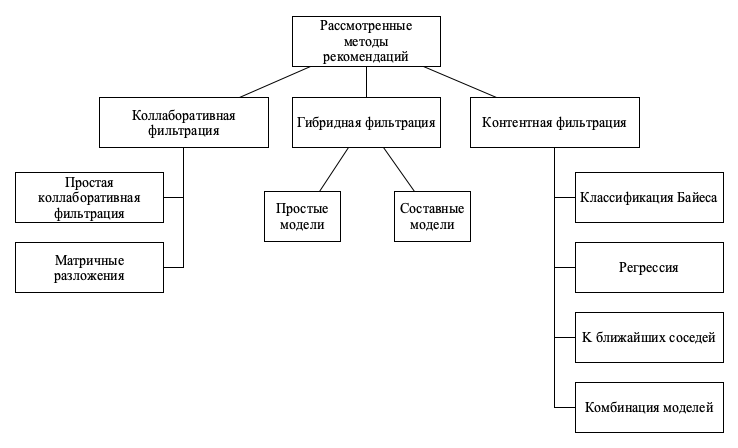
\includegraphics[width=\textwidth]{img/methods.png}
	\caption{
	    Классификация рассмотренных методов рекомендаций
	}
	\label{fig:methods}
\end{figure}
К коллаборативной фильтрации относятся алгоритмы рекомендаций, которые используют оценки данного пользователя и других, но не опираются на содержание рекомендуемых объектов.
Следовательно, если оценок рецептов от различных пользователей недостаточно, то рекомендации будут похожи на случайное угадывание.
Таким образом, данные алгоритмы будут более уместны в том случае, когда приложением пользуется достаточное количество людей, а если у приложения ещё недостаточно пользователей, то следует выбирать другие алгоритмы.
По этой же причине гибридная фильтрация также не выбрана для реализации.

Контентная фильтрация использует данные рекомендуемых объектов и прошлые оценки пользователя.
Поэтому реализация алгоритмов, основанных на ней, требует перевода рецептов в вектора.
Зато при этом отпадает потребность в оценках от разных пользователей.
Классификация Байеса предполагает бинаризацию значений вектора рецепта, вследствие которой часть данных потеряется, и также она хуже работает в случае, когда оценок более двух~\cite{aggarwal}.
Следовательно, её не стоит использовать.
Остальные методы могут быть применены и выбор между ними следует делать в зависимости от точности и эффективности модели рекомендаций.
Таким образом, для реализации выбраны методы <<$k$ ближайших соседей>> и регрессия с уменьшением размерности вектора рецепта.
Это методы с меньшей асимптотикой по сравнению с комбинацией рекомендательных моделей.
\section{Учёт возможностей пользователя}
Цель данной работы подразумевает, что рекомендации рецептов основаны не только на предпочтениях пользователя, но и на его возможностях.
Следовательно, необходимо фильтровать список рекомендованных пользователю рецептов.
Критерий, определяющий, стоит ли рекомендовать рецепт, заключается в следующем: количество ингредиентов этого рецепта, недоступных пользователю, должно быть не больше $N$.
Далее описан алгоритм учёта возможностей пользователя.
Вводятся следующие обозначения:
\begin{itemize}
    \item $A$ -- множество ингредиентов, которые у пользователя в наличии;
    \item $R$ -- множество рецептов;
    \item $I(r), r \in R$ -- множество ингредиентов рецепта $r$.
\end{itemize}
Условие соответствия рецепта критерию выбора имеет вид~\eqref{eq:select_cond}:
\begin{equation}
	\label{eq:select_cond}
	|\{x: x \in I(r), x \notin A\}| \leqslant N.
\end{equation}
Алгоритм фильтрации $R$ содержит следующие шаги:
\begin{itemize}
    \item создать пустой список $L$;
    \item перебрать все рецепты $r \in R$;
    \item если условие~\ref{eq:select_cond} выполнено, то добавить $r$ в список $L$;
    \item конец цикла по $r$.
\end{itemize}
В результате получается список рецептов, которые рекомендованы пользователю.
При необходимости критерий~\eqref{eq:select_cond} дополняется проверкой оценки и тегов, присвоенных рецепту.

\section*{Выводы}
\addcontentsline{toc}{section}{Выводы}
В результате данного раздела формализована задача рекомендательных систем и проанализированы способы формирования рекомендаций.
Рассмотрены методы, использующие только оценки данного пользователя и других, а также те методы, которые используют оценки данного пользователя и признаки рекомендуемых объектов.
Проведено сравнение представленных методов и на его основе обоснован выбор рекомендательного алгоритма.
Таким образом, получены все необходимые сведения для проектирования.
Следовательно, цель раздела достигнута.